The objective in the creation of this communication interface API was to develop an abstract interface that would allow any generic control algorithm or system (developed in Python or MATLAB) to be tested in a digital real-time simulation controller hardware-in-the-loop (CHIL) environment using the IEEE 1815 DNP3 communication protocol. The use of these APIs can streamline the testing process of algorithms designed to control grid-connected distributed energy resources (DERs) in a real-time simulation environment. This section focuses in the detailed description of the developed APIs' interface and how they facilitate the transfer of information between the user-defined control algorithms and the DNP3 module in charge of communicating values to the simulated power system inside the DRTS.
%subsection{Communication Interface}
As mentioned previously, the main goal behind the development of the proposed API was to create a flexible and easy-to-use interface that allows any generic control algorithm, developed either in Python or MATLAB, to be rapidly tested in a real-time simulation environment using the DNP3 protocol. The API is in charge of exchanging information between the DNP3 module and the algorithm under test. To accomplish this, the API uses TCP/IP sockets, for inter-process communication, that transfers data and commands to and from the algorithm running in the controller under test, the database management server (DMS), and the DNP3 module that act as a master device. 

% \begin{figure}[!ht]
%     \centering
%     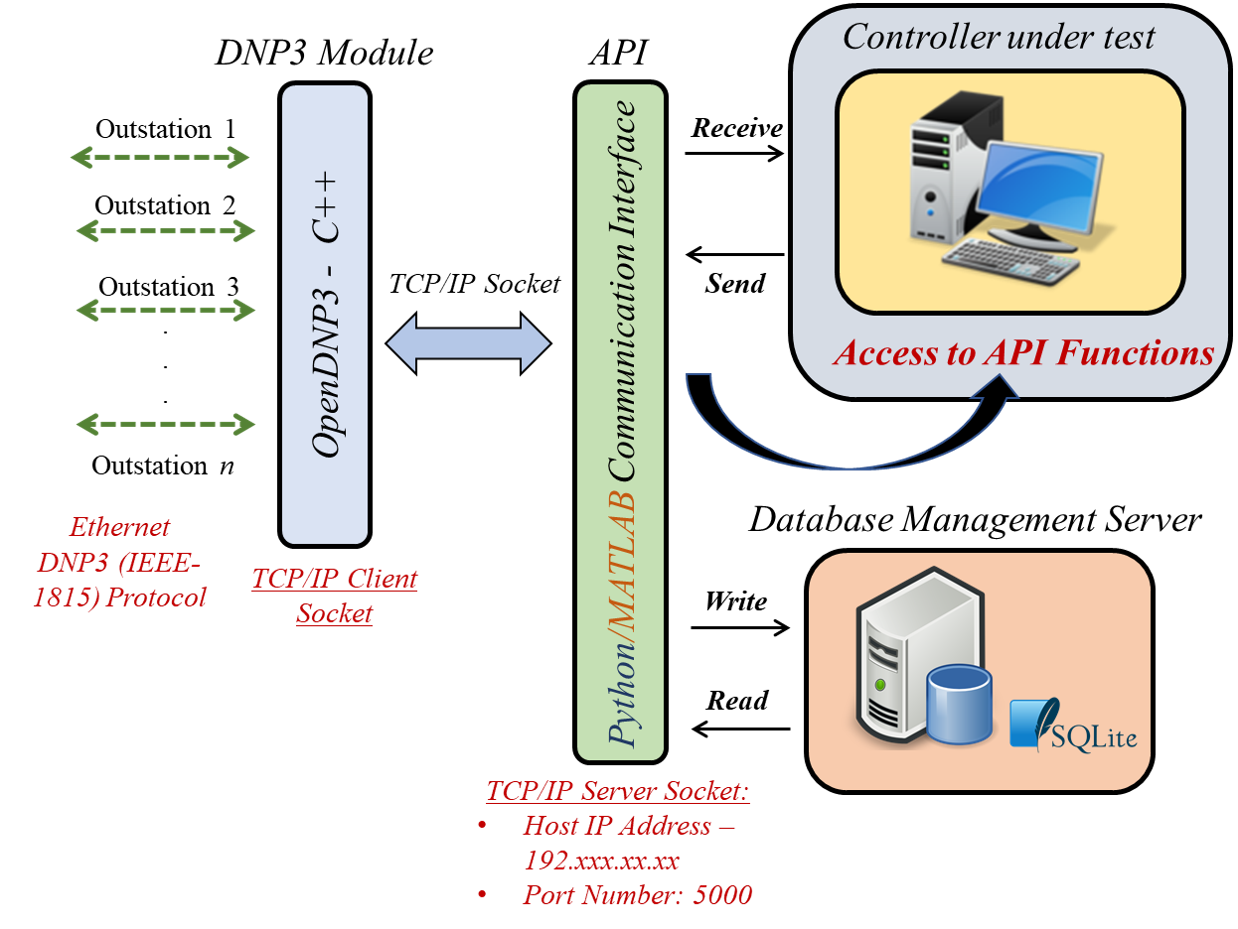
\includegraphics[width = 1.0\linewidth]{figs_juan/apiblocks.png}
%     \caption{Block diagram demonstrating how the information is exchanged between the Python/MATLAB APIs, the DNP3 module, the DMS, and the DNP3 outstations simulated inside the DRTS.}
%     \label{fig:apiblocks}
% \end{figure}


The DNP3 module is implemented using a modified version of the open source application called \textit{OpenDNP3}. The original version of OpenDNP3 was modified to include the following features:

\begin{itemize}
    \item Communicate directly with smart-meter models (outstations) deployed in the power system model inside the DRTS. 
    
    \item DNP3 modules operate in \textit{unsolicited response} mode (Can also be configured to work in \textit{event polling} mode). 
    
    \item Read and write data to a database management server (DMS) deployed as an external system using SQLite. This module has the capability to send data directly to outstations and read data from the DMS.
\end{itemize}

% A detailed description of all the five functions that are part of the proposed API is presented below. These functions are the following:
% \begin{enumerate}

%     \item \textit{create\_socket}: This function is in charge of creating the TCP/IP socket IPC connection between the DNP3 module and the algorithm executing in the controller under test. The parameters of this function are the host IP address (where the DNP3 master module is running) and the socket port number where the server is going to reside. This function returns the socket client connected, i.e., where the data is being transmitted.
    
%     \item \textit{create\_database\_conn}: This function is in charge of creating the connection to the database management server (DMS) where all the data received from the DNP3 outstations (smart-meters) is being recorded. The only input parameter to this function is the name or path to where the SQLite database resides. If the connection is successful, the function returns the database connection, if not returns \textit{error}.
    
%     \item \textit{check\_database\_status}: This function has the capability of checking the status of the database. It has two input parameters. The first one indicates the last time the database was modified. Based on this modification time, this function returns True if the modification time is not the same as the current modification or False otherwise. The second input parameter is needed to identify the name of the database undergoing the checking operation.
    
%     \item \textit{read\_database}: This function provides the ability to retrieve any value from the database management server (DMS). The input parameters of this function are the table to read inside the database and the established connection to a specific database. In other words, the output of the \textit{create\_database\_conn} needs to be passed in as the second parameter. This function returns the values stored in the specified table inside the respective database.
    
%     \item \textit{send\_data}: This function in charge of sending the control values from the controller under test to the grid-connected DERs simulated inside the DRTS. The inputs of this function are: a) the specific control values to send to the DRTS, b) the data format of these values, c) the index number of the outstation where the control values need to be sent.
%     \vspace{-1mm}
% \end{enumerate}
It is important to mention that the proposed API was designed to work with SQLite databases due to SQLite great portability and excellent compatibility across multiple platforms such as Windows and Linux operating systems. Nevertheless, if needed this API can be easily modified to be compatible with other databases such as Microsoft SQL and MySQL. The next section presents an example use case related to an energy management solution designed to control DERs in microgrid setting simulated in a real-time environment.


% The pseudocode presented below describes how the developed interfaces can be used with any generic control algorithm. In other words, illustrates an example use case showing how any generic code can reference the API functions developed and how to use them for testing procedures. 

% \begin{algorithm}[H]
%  \caption{Example Usage of API Functions}
%  \begin{algorithmic}[1]
%  \renewcommand{\algorithmicrequire}{\textbf{Input: }}
%  \renewcommand{\algorithmicensure}{\textbf{Output:}}
%  \REQUIRE \(N/A\)
%  \ENSURE  \(controls\)
%  \\ \textit{Initialisation} : database\_name, data\_format\\
%  host\_IP, port\_Number, time\_modified\\
%   \STATE socket\_client $\leftarrow$ \textit{create\_socket}(host\_IP, port\_Number)
%   \STATE database\_conn $\leftarrow$ \textit{create\_database\_conn}(database\_name)
%   \WHILE{(running\_criteria)}
%   \IF {(\textit{check\_database}(time\_modified, database\_conn))}
%   \STATE data\_read $\leftarrow$
%   \textit{read\_database}(table\_name, 
%   \\ database\_conn)
%   \STATE controls $\leftarrow$ \textbf{Algorithm Execution(data\_read)}
%   \STATE \textit{send\_data}(values, data\_format, outstation\_index)
%   \ELSE 
%   \STATE \textit{CONTINUE}
%   \ENDIF
%   \ENDWHILE
%  \RETURN $controls$
%  \end{algorithmic}
%  \end{algorithm}
 